\subsection{Elementary Operations on Sets}

\exercise{1}{
    Prove all the displayed formulas in this section and visualize them using Venn diagrams.
}
\sol{
    \newcommand*{\comproof}[2]{
        \ali{
            x \in A #1 B &\bic x \in A #2 x \in B \\
            &\bic x \in B #2 x \in A \\
            &\bic x \in B #1 A,
        }
    }
    \newcommand*{\assocproof}[2]{
        \ali{
            (A #1 B ) #1 C &\bic x \in A #1 B #2 x \in C \\
            &\bic (x \in A #2 x \in B) #2 x \in C \\
            &\bic x \in A #2 x \in B #2 x \in C \\
            &\bic x \in A #2 (x \in B #2 x \in C) \\
            &\bic x \in A #2 x \in B #1 C \\
            &\bic x \in A #1 (B #1 C),
        }
    }
    For commutivity, Venn diagrams are not very useful.
    \qproof{
        For all $x$, we have that
        \comproof{\cap}{\land}
        which shows that $A \cap B = B \cap A$.
        Similarly, we have that
        \comproof{\cup}{\lor}
        which proves that $A \cup B = B \cup A$.
    }

    Venn diagrams also provide no insight for associativity.
    \qproof{
        Again, for any $x$, we have that
        \assocproof{\cap}{\land}
        showing that $(A \cap B) \cap C = A \cap (B \cap C)$.
        Likewise, we have
        \assocproof{\cup}{\lor}
        and hence $(A \cup B) \cup C = A \cup (B \cup C)$.
    }

    \newcommand{\venndiag}[7]{
        \begin{center}
            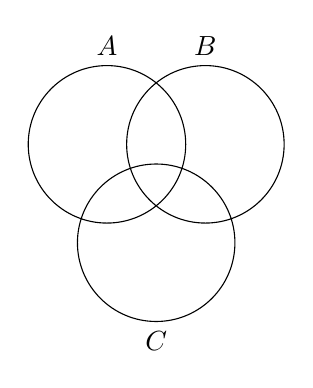
\begin{tikzpicture}[fill=gray]
                \def\bx{1.25}
                \def\cy{-1.25}
                \def\circA{(0,0) circle (1)}
                \def\circB{(\bx,0) circle (1)}
                \def\circC{(\bx/2,\cy) circle (1)}
                \def\vennrect{(-1,\cy-1) rectangle (\bx+1,1)}
                \def\@true{1}

                % A only
                \ifx1#1
                    \begin{scope}
                        \clip \vennrect \circB;
                        \clip \vennrect \circC;
                        \fill \circA;
                    \end{scope}
                \fi

                % B only
                \ifx1#2
                    \begin{scope}
                        \clip \vennrect \circA;
                        \clip \vennrect \circC;
                        \fill \circB;
                    \end{scope}
                \fi

                % C only
                \ifx1#3
                    \begin{scope}
                        \clip \vennrect \circA;
                        \clip \vennrect \circB;
                        \fill \circC;
                    \end{scope}
                \fi

                % A and B only
                \ifx1#4
                    \begin{scope}
                        \clip \vennrect \circC;
                        \clip \circA;
                        \clip \circB;
                        \fill \circA;
                    \end{scope}
                \fi

                % A and C only
                \ifx1#5
                    \begin{scope}
                        \clip \vennrect \circB;
                        \clip \circA;
                        \clip \circC;
                        \fill \circA;
                    \end{scope}
                \fi

                % B and C only
                \ifx1#6
                    \begin{scope}
                        \clip \vennrect \circA;
                        \clip \circB;
                        \clip \circC;
                        \fill \circB;
                    \end{scope}
                \fi

                % A and B and C
                \ifx1#7
                    \begin{scope}
                        \clip \circA;
                        \clip \circB;
                        \clip \circC;
                        \fill \circA;
                    \end{scope}
                \fi

                % Draw circles and labels
                \draw \circA (0,1)  node [text=black,above] {$A$}
                \circB (\bx,1)  node [text=black,above] {$B$}
                \circC (\bx/2,\cy-1)  node [text=black,below] {$C$};
            \end{tikzpicture}
        \end{center}
    }
    \newcommand*{\distproof}[4]{
        \ali{
            x \in A #1 (B #2 C) &\bic x \in A #3 (x \in B #4 x \in C) \\
            &\bic (x \in A #3 x \in B) #4 (x \in A #3 x \in C) \\
            &\bic x \in A #1 B #4 x \in A #1 C \\
            &\bic x \in (A #1 B) #2 (A #1 C),
        }
    }
    For distributivity, Venn diagrams \emph{do} provide insight.
    The Venn diagram for the distributive identity $A \cap (B \cup C) = (A \cap B) \cup (A \cap C)$ is shown below:
    \venndiag{0}{0}{0}{1}{1}{0}{1}
    A proof of this follows directly from the distributivity of logical conjunction.
    \qproof{
        For all $x$, we have
        \distproof{\cap}{\cup}{\land}{\lor}
        which proves the result.
    }
    Likewise, the Venn diagram for $A \cup (B \cap C) = (A \cup B) \cap (A \cup C)$ is shown below:
    \venndiag{1}{0}{0}{1}{1}{1}{1}
    This time, the proof follows directly from the distributivity of logical disjunction.
    \qproof{
        For every $x$, we have that
        \distproof{\cup}{\cap}{\lor}{\land}
        proving the desired result.
    }

    \newcommand\demorgproof[4]{
        \ali{
            x \in C - (A #1 B) &\bic x \in C \land x \notin A #1 B \\
            &\bic x \in C \land \lnot (x \in A #1 B) \\
            &\bic x \in C \land \lnot (x \in A #2 x \in B) \\
            &\bic x \in C \land (x \notin A #3 x \notin B) \\
            &\bic (x \in C \land x \notin A) #3 (x \in C \land x \notin B) \\
            &\bic x \in C - A #3 x \in C - B \\
            &\bic x \in (C - A) #4 (C - B),
        }
    }
    Regarding the two DeMorgan laws, proofs of these rely on the DeMorgan and distributive laws of logic.
    First, we have $C - (A \cap B) = (C - A) \cup (C - B)$:
    \venndiag{0}{0}{1}{0}{1}{1}{0}
    \qproof{
        For all $x$,
        \demorgproof{\cap}{\land}{\lor}{\cup}
        of course showing the result.
    }
    The other DeMorgan law is of course $C - (A \cup B) = (C - A) \cap (C - B)$:
    \venndiag{0}{0}{1}{0}{0}{0}{0}
    \qproof{
        Again, for all $x$, we have
        \demorgproof{\cup}{\lor}{\land}{\cap}
        which proves the result.
    }
}

\exercise{2}{
    Prove:
    \begin{enumerate}
        \item[(a)] $A \ss B$ if and only if $A \cap B = A$ if and only if $A \cup B = B$ if and only if $A - B = \es$.
        \item[(b)] $A \ss B \cap C$ if and only if $A \ss B$ and $A \ss C$.
        \item[(c)] $B \cup C \ss A$ if and only if $B \ss A$ and $C \ss A$.
        \item[(d)] $A - B = (A \cup B) -B = A - (A \cap B)$.
        \item[(e)] $A \cap B = A - (A - B)$.
        \item[(f)] $A - (B - C) = (A - B) \cup (A \cap C)$.
        \item[(g)] $A = B$ if and only if $A \sd B = \es$.
    \end{enumerate}
}
\sol{
    TODO
}

\exercise{3}{
    For each of the following (false) statements draw a Venn diagram in which it fails:
    \begin{enumerate}
        \item[(a)] $A - B = B - A$.
        \item[(b)] $A \cap B \pss A$.
        \item[(c)] $A \ss B \cup C$ implies $A \ss B$ or $A \ss C$.
        \item[(d)] $B \cap C \ss A$ implies $B \ss A$ or $C \ss A$.
    \end{enumerate}
}
\sol{
    TODO
}

\exercise{4}{
    Let $A$ be a set; show that a ``complement'' of $A$ does not exist.
    (The ``complement'' of $A$ is the set of all $x \notin A$.)
}
\sol{
    TODO
}

\exercise{5}{
    Let $S \neq \es$ and $A$ be sets.
    \begin{enumerate}
        \item[(a)] Set $T_1 = \braces{Y \in \pset{A} \where \text{$Y = A \cap X$ for some $X \in S$}}$, and prove $A \cap \bigcup S = \bigcup T_1$ (generalized distributive law).
        \item[(b)] Set $T_2 = \braces{Y \in \pset{A} \where \text{$Y = A - X$ for some $X \in S$}}$, and prove
            \gath{
                A - \bigcup S = \bigcap T_2 \\
                A - \bigcap S = \bigcup T_2
            }
            (generalized De Morgan's laws).
    \end{enumerate}
}
\sol{
    TODO
}

\exercise{6}{
    Prove that $\bigcap S$ exists for all $S \neq \es$.
    Where s the assumption that $S \neq \es$ used in the proof?
}
\sol{
    TODO
}